\documentclass[10pt,handout]{beamer}

\usepackage[french]{babel}
\usepackage[T1]{fontenc}
\usepackage[utf8]{inputenc}
\usepackage[
    left = \flqq{},%
    right = \frqq{},%
    leftsub = \flq{},%
    rightsub = \frq{} %
]{dirtytalk} 	% for \say{}
\usepackage{xcolor} 	% for color text
\usepackage{csquotes}
\usepackage{amssymb}
\usepackage{mathtools}
\usepackage{array}

% Bout de code
\usepackage{listings}
\usepackage{color}

\definecolor{mygreen}{rgb}{0,0.6,0}
\definecolor{mygray}{rgb}{0.5,0.5,0.5}
\definecolor{mymauve}{rgb}{0.58,0,0.82}

\lstset{
  backgroundcolor=\color{white},   % choose the background color; you must add \usepackage{color} or \usepackage{xcolor}; should come as last argument
  basicstyle=\footnotesize,        % the size of the fonts that are used for the code
  breakatwhitespace=false,         % sets if automatic breaks should only happen at whitespace
  breaklines=true,                 % sets automatic line breaking
  captionpos=b,                    % sets the caption-position to bottom
  commentstyle=\color{mygreen},    % comment style
  deletekeywords={...},            % if you want to delete keywords from the given language
  escapeinside={\%*}{*)},          % if you want to add LaTeX within your code
  extendedchars=true,              % lets you use non-ASCII characters; for 8-bits encodings only, does not work with UTF-8
  firstnumber=0,                   % start line enumeration with line 1000
  frame=single,	                   % adds a frame around the code
  keepspaces=true,                 % keeps spaces in text, useful for keeping indentation of code (possibly needs columns=flexible)
  keywordstyle=\color{blue},       % keyword style
  %language=C++,                    % the language of the code
  morekeywords={*,...},            % if you want to add more keywords to the set
  numbers=left,                    % where to put the line-numbers; possible values are (none, left, right)
  numbersep=5pt,                   % how far the line-numbers are from the code
  numberstyle=\tiny\color{mygray}, % the style that is used for the line-numbers
  rulecolor=\color{black},         % if not set, the frame-color may be changed on line-breaks within not-black text (e.g. comments (green here))
  showspaces=false,                % show spaces everywhere adding particular underscores; it overrides 'showstringspaces'
  showstringspaces=false,          % underline spaces within strings only
  showtabs=false,                  % show tabs within strings adding particular underscores
  stepnumber=1,                    % the step between two line-numbers. If it's 1, each line will be numbered
  stringstyle=\color{mymauve},     % string literal style
  tabsize=2,	                   % sets default tabsize to 2 spaces
  literate=
  {á}{{\'a}}1 {é}{{\'e}}1 {í}{{\'i}}1 {ó}{{\'o}}1 {ú}{{\'u}}1
  {Á}{{\'A}}1 {É}{{\'E}}1 {Í}{{\'I}}1 {Ó}{{\'O}}1 {Ú}{{\'U}}1
  {à}{{\`a}}1 {è}{{\`e}}1 {ì}{{\`i}}1 {ò}{{\`o}}1 {ù}{{\`u}}1
  {À}{{\`A}}1 {È}{{\'E}}1 {Ì}{{\`I}}1 {Ò}{{\`O}}1 {Ù}{{\`U}}1
  {ä}{{\"a}}1 {ë}{{\"e}}1 {ï}{{\"i}}1 {ö}{{\"o}}1 {ü}{{\"u}}1
  {Ä}{{\"A}}1 {Ë}{{\"E}}1 {Ï}{{\"I}}1 {Ö}{{\"O}}1 {Ü}{{\"U}}1
  {â}{{\^a}}1 {ê}{{\^e}}1 {î}{{\^i}}1 {ô}{{\^o}}1 {û}{{\^u}}1
  {Â}{{\^A}}1 {Ê}{{\^E}}1 {Î}{{\^I}}1 {Ô}{{\^O}}1 {Û}{{\^U}}1
  {Ã}{{\~A}}1 {ã}{{\~a}}1 {Õ}{{\~O}}1 {õ}{{\~o}}1
  {œ}{{\oe}}1 {Œ}{{\OE}}1 {æ}{{\ae}}1 {Æ}{{\AE}}1 {ß}{{\ss}}1
  {ű}{{\H{u}}}1 {Ű}{{\H{U}}}1 {ő}{{\H{o}}}1 {Ő}{{\H{O}}}1
  {ç}{{\c c}}1 {Ç}{{\c C}}1 {ø}{{\o}}1 {å}{{\r a}}1 {Å}{{\r A}}1
  {€}{{\euro}}1 {£}{{\pounds}}1 {«}{{\guillemotleft}}1
  {»}{{\guillemotright}}1 {ñ}{{\~n}}1 {Ñ}{{\~N}}1 {¿}{{?`}}1
}

\usetheme{Frankfurt}
\usetheme{CambridgeUS}
\usetheme{JuanLesPins}
%\usetheme{Montpellier}
%\usetheme{Madrid}

\usecolortheme{dolphin}

\useinnertheme{circles}
\usefonttheme{structurebold}
\useoutertheme{default}

%\hypersetup{pdfpagemode=FullScreen}

\title[Chemins spécifiques]{Chemins spécifiques pour la classification dans les réseaux de neurones profonds}
\author[Bouzidi, Elhouiti, Kezzoul]{Bouzidi Belkassim - Elhouiti Chakib - Kezzoul Massili \\}
\institute[]{Université de Montpellier}
\date{\today}

% Pour inserer une frame de sommaire avant chaque debut de section
\AtBeginSection[]
{
  \placelogofalse
  \begin{frame}
    \tableofcontents[hideothersubsections,currentsection,subsectionstyle=show/shaded/hide]
  \end{frame}
  \placelogotrue
}

% Mettre les listes en triangle
\setbeamertemplate{itemize item}[triangle]

%Insertion d'un logo
\newif\ifplacelogo % create a new conditional
\placelogotrue % set it to true
\logo{\ifplacelogo
\includegraphics[height=12mm]{img/univ-montpellier.png}\fi}

%------------------------------------------------------%
% page de titre
%------------------------------------------------------%
\begin{document}

\placelogofalse
\begin{frame}
	\titlepage
\end{frame}

\placelogotrue

\section{Introduction}
\subsection{Les réseaux de neurones profonds}
\placelogofalse
\begin{frame}{Présentation des réseaux de neurones}
    \begin{block}{}
        Les réseaux de neurones sont constitués de plusieurs couches consécutives de neurones interconnectées.
    \end{block}

    \makebox[\textwidth]{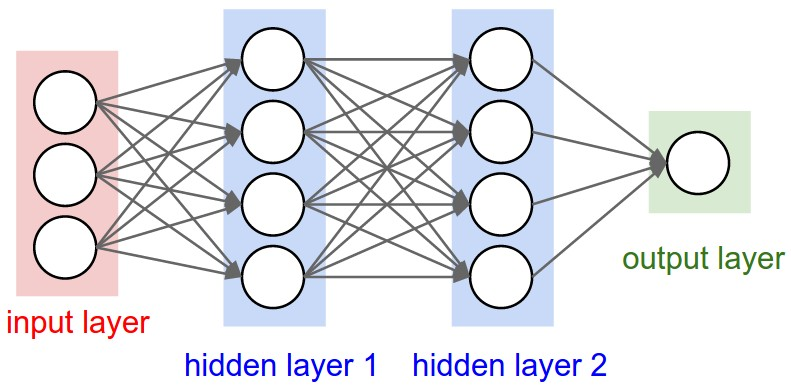
\includegraphics[width=0.5\textwidth]{img/ann-dense.jpg}}

\end{frame}

\begin{frame}{Fonctionnement}
    \makebox[\textwidth]{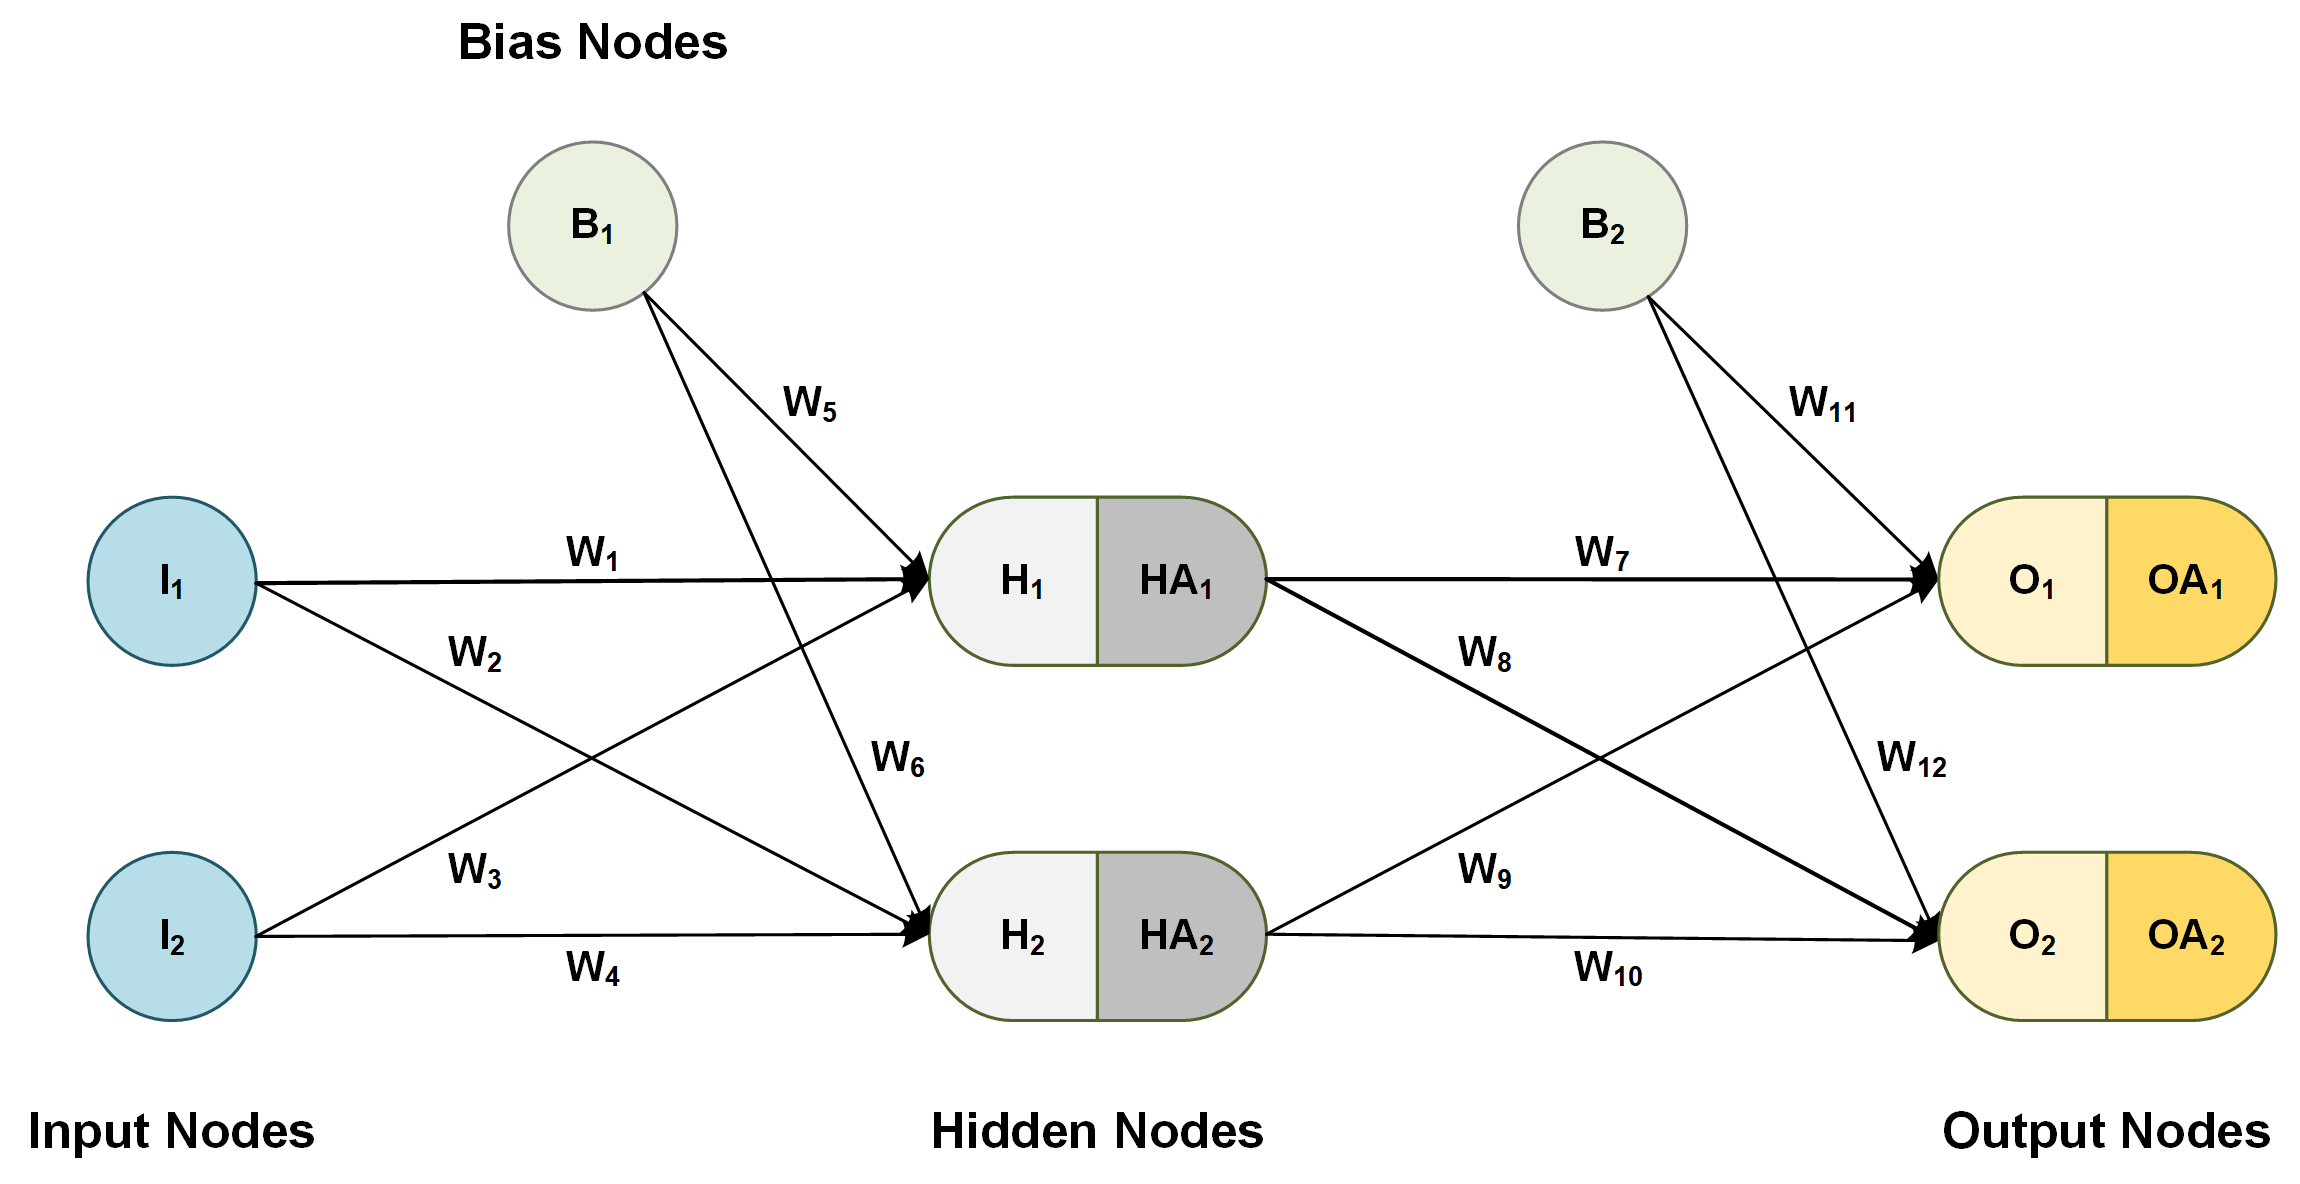
\includegraphics[width=1.\textwidth]{img/ann-biais-poids.png}}
\end{frame}

\begin{frame}{Boite noire}
    \makebox[\textwidth]{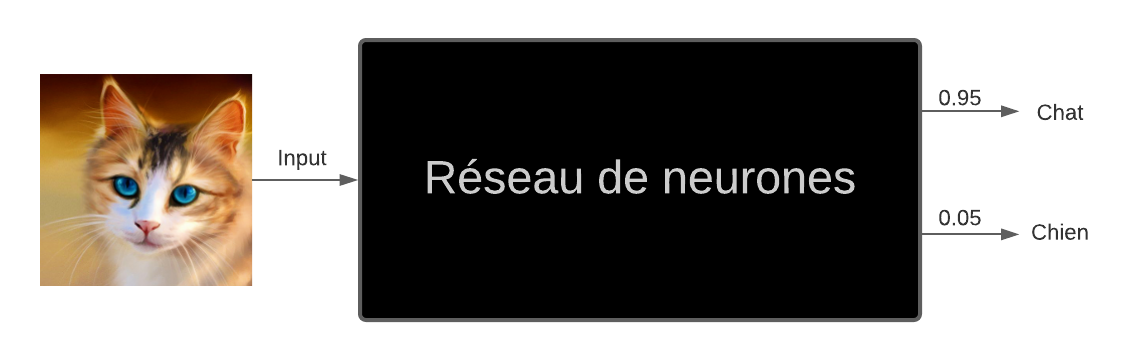
\includegraphics[width=0.9\textwidth]{img/black-box.png}}

    \makebox[\textwidth]{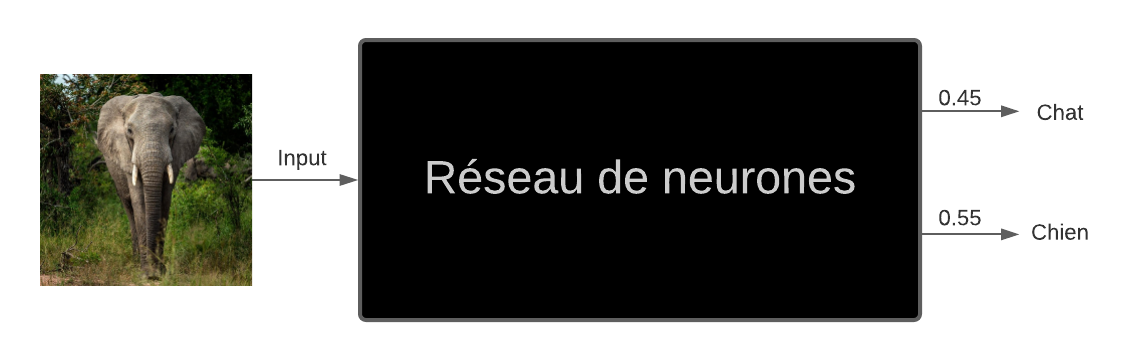
\includegraphics[width=0.9\textwidth]{img/black-box2.png}}
\end{frame}
\placelogotrue

\subsection{Problèmatique}
\begin{frame}{Problèmatique}
    \begin{block}{Objectifs}
        L'objectif est de comprendre le fonctionnement interne d'un réseau de neurones et de repérer des signatures d'activations.

        \begin{itemize}
        \item À partir de quelle couche le modèle change de comportement pour reconnaître une image ?
        \item Les signatures des images de \textit{7}, sont-elles différentes de ceux des \textit{1} ?
        \item Si on passe une image de \textit{3} au modèle, à quoi va ressembler sa signature ?
        \end{itemize}    
    \end{block}
        
\end{frame}

\subsection{Solution proposée}
\begin{frame}{Solution proposée}
    \begin{itemize}
        \item Construire des réseaux de neurones.
        \item Récupérer, pour chaque donnée, la sortie des couches cachées.
        \item Extraire les signatures grâce à des algorithmes de \textit{clustering}.
        \item Réaliser une interface de visualisation en utilisant différentes techniques.
    \end{itemize}
\end{frame}

\section{Organisation}
\placelogofalse
\begin{frame}{Organisation du projet}
    \makebox[\textwidth]{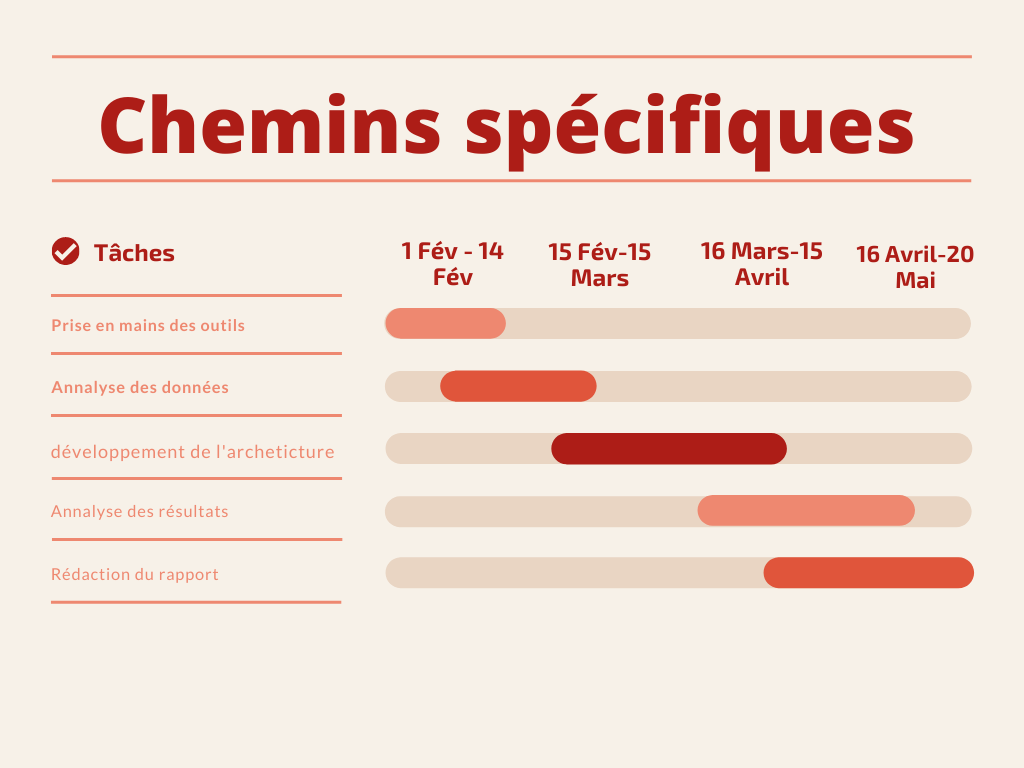
\includegraphics[width=0.8\textwidth]{img/diagramme_gantt.png}}
\end{frame}
\placelogotrue

\section{Analyse des données}
\placelogofalse
\begin{frame}{Le jeu de données}
    \begin{block}{Mixed National Institute of Standards and Technology}
       Base de données composée de \textit{70000} images de chiffre manuscrit.
    \end{block}
    \makebox[\textwidth]{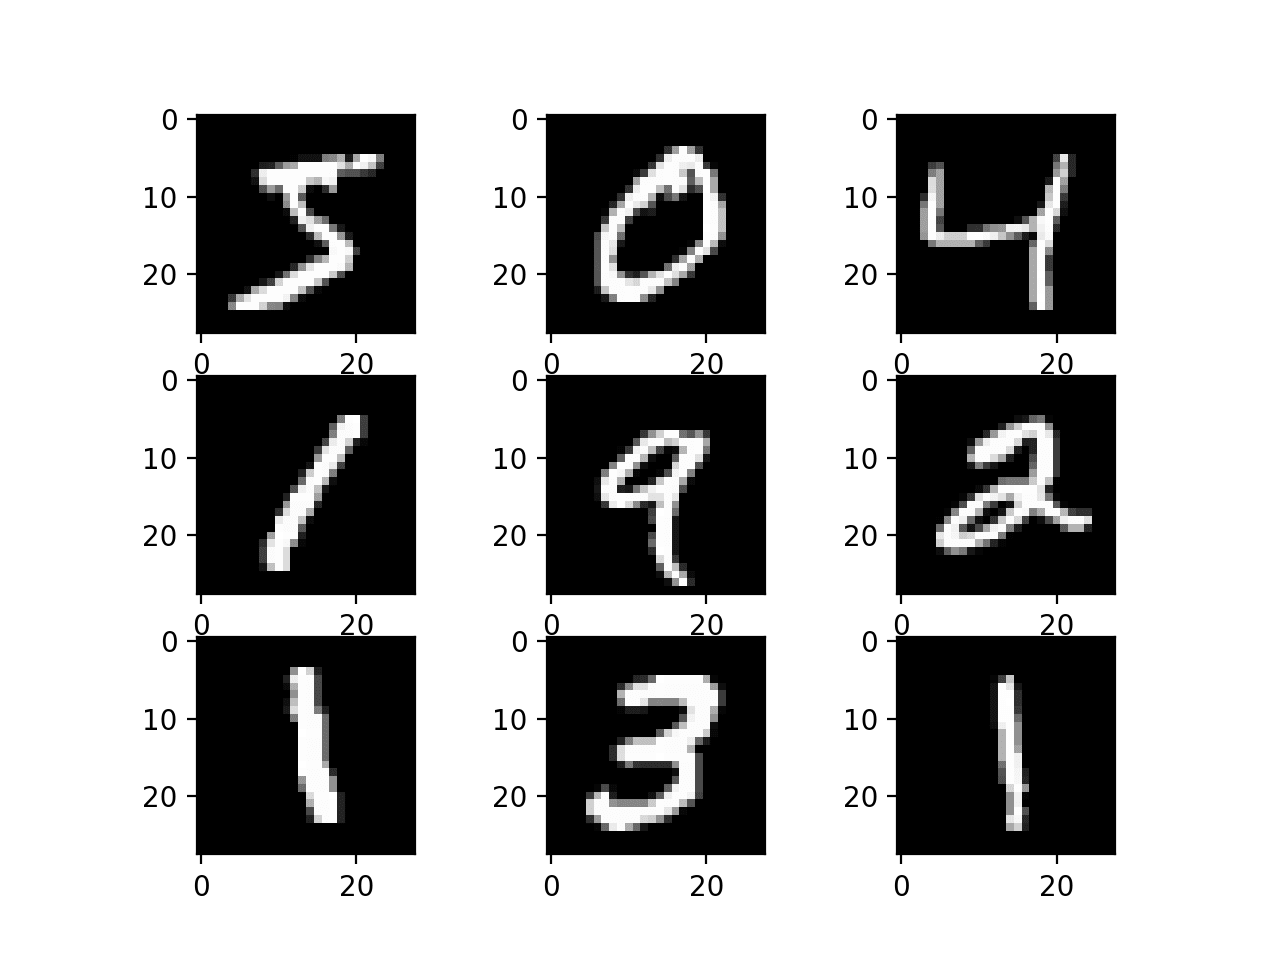
\includegraphics[width=0.7\textwidth]{img/mnist.png}}
\end{frame}
\placelogotrue
 
\subsection{Seléction des données}

\begin{frame}{Seléction des données}
    \begin{itemize}
        \item Garder un nombre précis d’images pour un ensemble de chiffres définis.
        \item Faciliter la phase de développement.
        \item Pouvoir mieux visualiser les résultats sur un petit ensemble de données.
    \end{itemize}
\end{frame}

\subsection{Prétraitement}

\placelogofalse
\begin{frame}{Prétraitement}
\begin{block}{Scaling}
    Normalisation: Mettre les valeurs des images entre 0 et 1 au lieu de 0 et 255.
\end{block}

\begin{block}{Flattening}
    Applatir les images pour avoir un tableau à une seule dimension au lieu d’une matrice.
\end{block}

\begin{block}{One-hot encoding}
    Transformation des labels en un vecteur binaire contenant que des 0 et des 1.
    \begin{itemize}
        \item Pour un 1 $\implies$ [1,0,0].
        \item Pour un 3 $\implies$ [0,1,0].
        \item Pour un 7 $\implies$ [0,0,1].
    \end{itemize}
\end{block}
\end{frame}
\placelogotrue

\section{Développement de l’architecture}

\subsection{Technologies utilisées}

\placelogofalse
\begin{frame}{Jupyter notebook}
    \makebox[\textwidth]{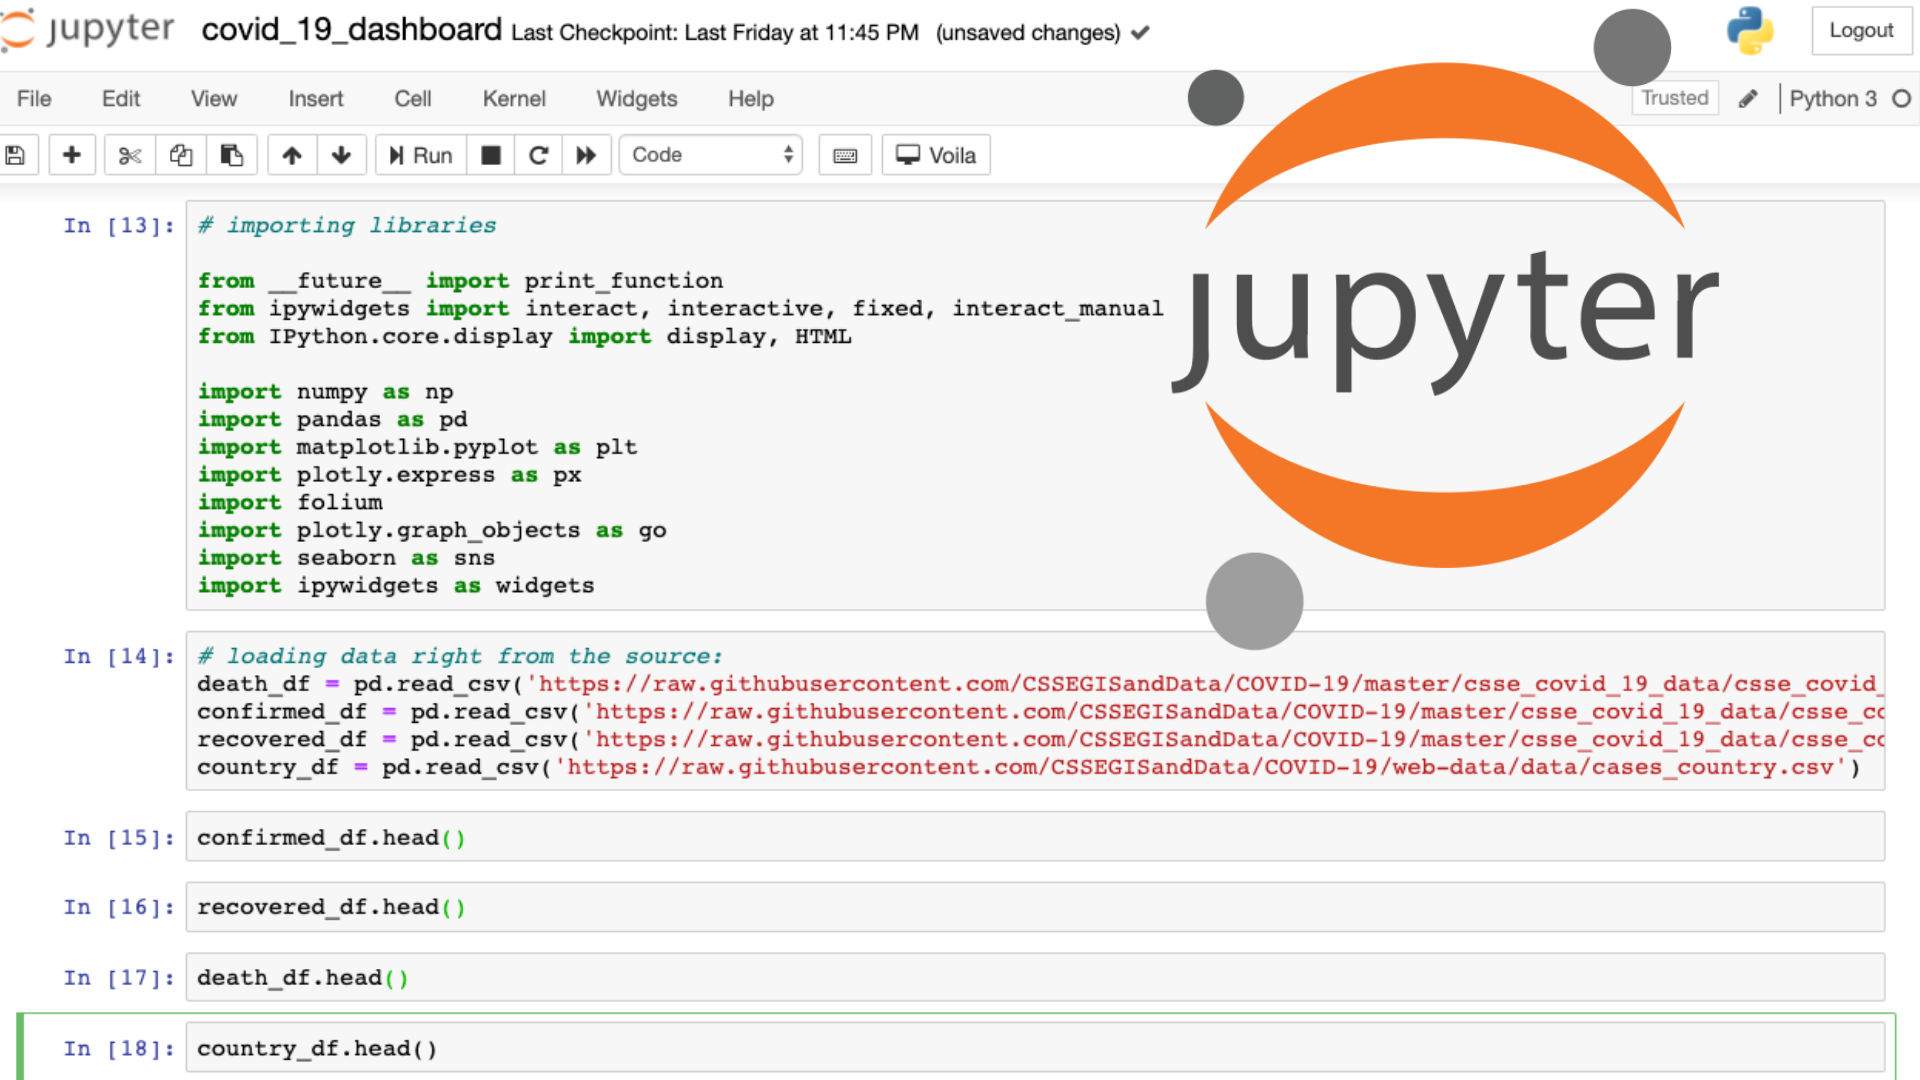
\includegraphics[width=0.9\textwidth]{img/jupyter.png}}
\end{frame}
\placelogotrue

\begin{frame}{Tensorflow, Keras}
    \makebox[\textwidth]{
\includegraphics[width=0.9\textwidth]{img/tensor&keras.jpg}}
\end{frame}

\placelogofalse
\begin{frame}{Voilà}
    \begin{figure}[h]
        \begin{minipage}[c]{.46\linewidth}
        \centering
        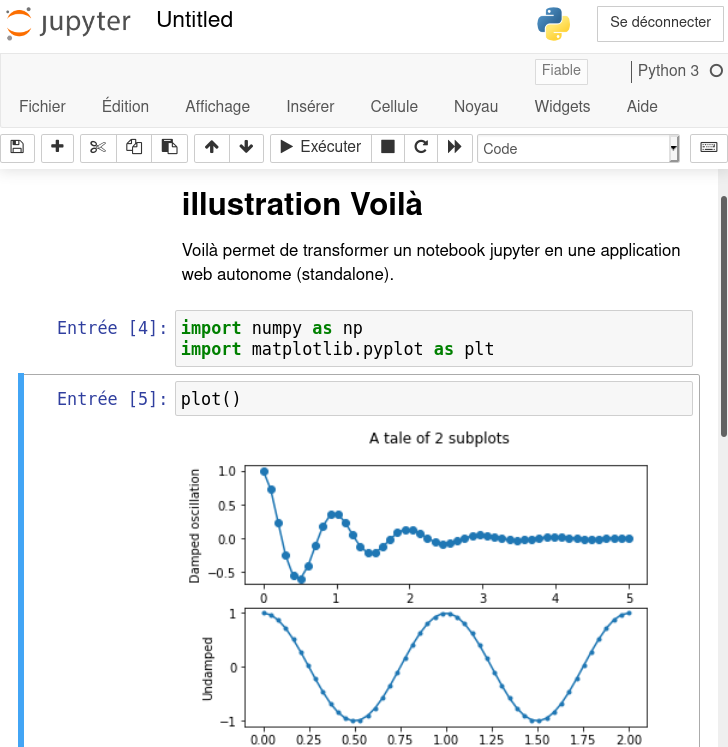
\includegraphics[width=1.0\textwidth]{img/voila1.png}
        \end{minipage}
        \hfill%
        \begin{minipage}[c]{.46\linewidth}
        \centering
        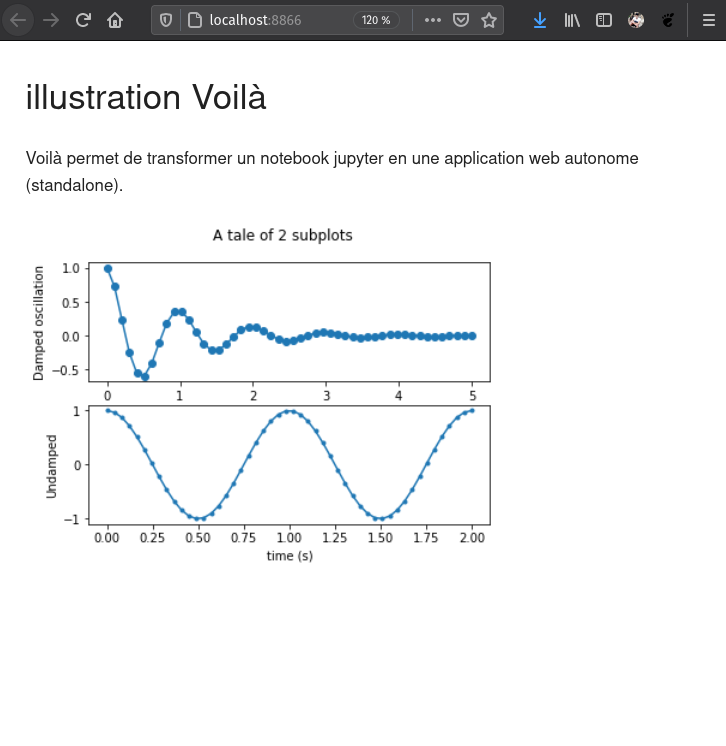
\includegraphics[width=1.0\textwidth]{img/voila2.png}
        \end{minipage}
    \end{figure}
\end{frame} 

\subsection{Modèle d'apprentissage}
\begin{frame}{Création du modèle}
    \begin{block}{Modèle}
        \begin{itemize}
            \item 2 couches cachées;
            \item 32 neurones pour la première;
            \item 64 pour la deuxième;
            \item fonction d'activation \textit{relu} pour les couches internes;
            \item et \textit{softmax} pour la dernière couche.
        \end{itemize}
    \end{block}
    \vspace{5mm}
    \makebox[\textwidth]{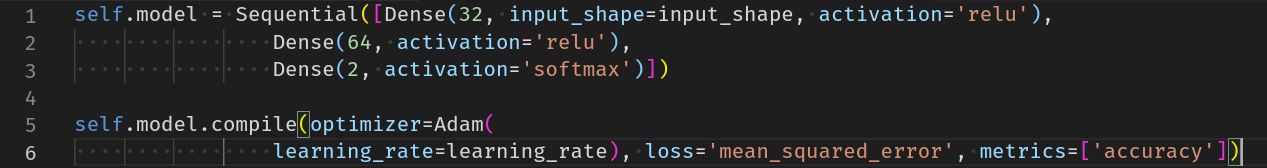
\includegraphics[width=0.9\textwidth]{img/build-model-code.png}}
\end{frame}
\placelogotrue 

\placelogofalse 
\begin{frame}{Clustering}
    \begin{block}{K-means}
        \textbf{K-means} prend en paramètres les données et un certain $K$ donnée par l’utilisateur, puis construit $K$ clusters qui regroupent les données qui sont proches (en terme de distance euclidienne).
    \end{block}
    \makebox[\textwidth]{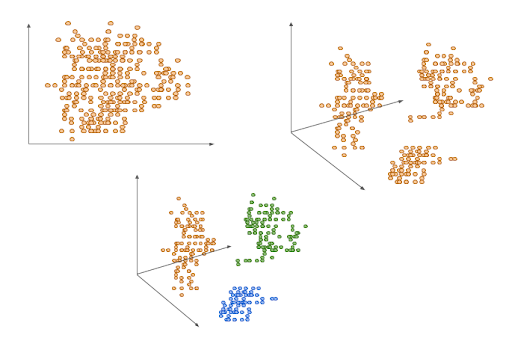
\includegraphics[width=0.6\textwidth]{img/kmeans.png}}
\end{frame}
\placelogotrue 

\begin{frame}{Choix du $K$}
    \begin{block}{Choix du $K$}
        Concrétement, cette méthode consiste à calculer pour un clustering, la moyenne du score \textit{Silhouette} de chaque point.
    \end{block}
    \makebox[\textwidth]{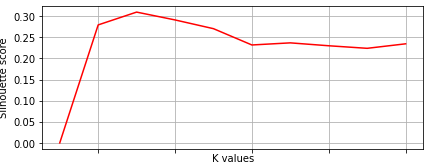
\includegraphics[width=0.8\textwidth]{img/silhouette.png}}
\end{frame}

\subsection{Interface de visualisation}
\placelogofalse
\begin{frame}{UMAP}
    \begin{block}{UMAP}
        (Uniform Manifold Approximation and Projection) Utilise des algorithmes de mise en page graphique pour organiser les données dans
        un espace de faible dimension.
    \end{block}
    \makebox[\textwidth]{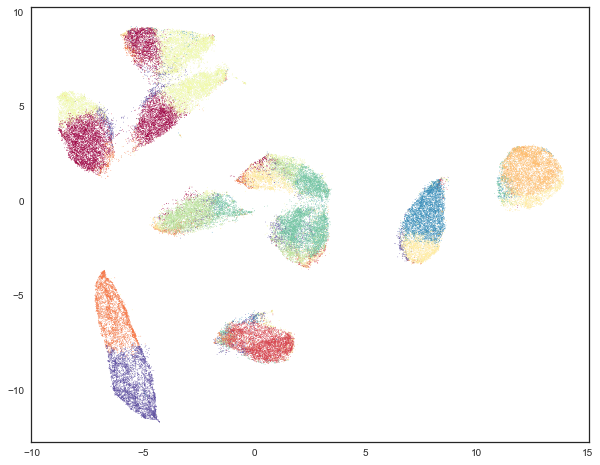
\includegraphics[width=0.6\textwidth]{img/UMAP.png}}
\end{frame}
\placelogotrue

\begin{frame}{Diagramme de Sankey}
    \begin{block}{}
        Un diagramme de Sankey est un type de diagramme de flux dans lequel la largeur des flèches
        est proportionnelle au flux représenté.
    \end{block}
    \makebox[\textwidth]{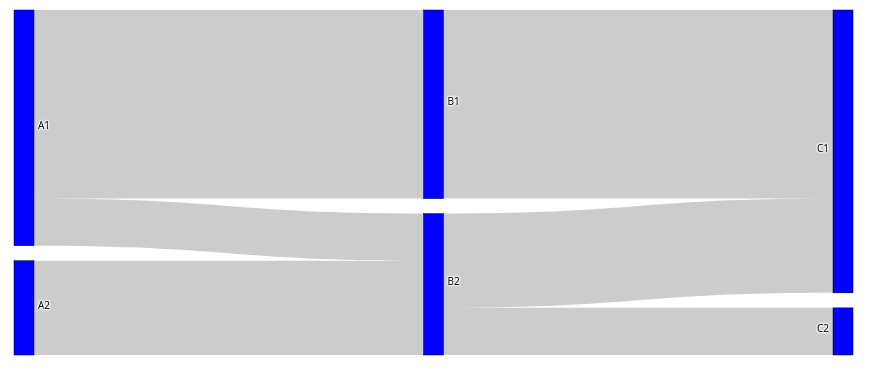
\includegraphics[width=0.6\textwidth]{img/sankey.png}}
\end{frame}
\placelogofalse
\begin{frame}{Application web}
    \begin{block}{Page web}
        Transformation d'un Jupyter notebook contenant les différentes visualisations et faisant le lien entre eux.
    \end{block}
    \makebox[\textwidth]{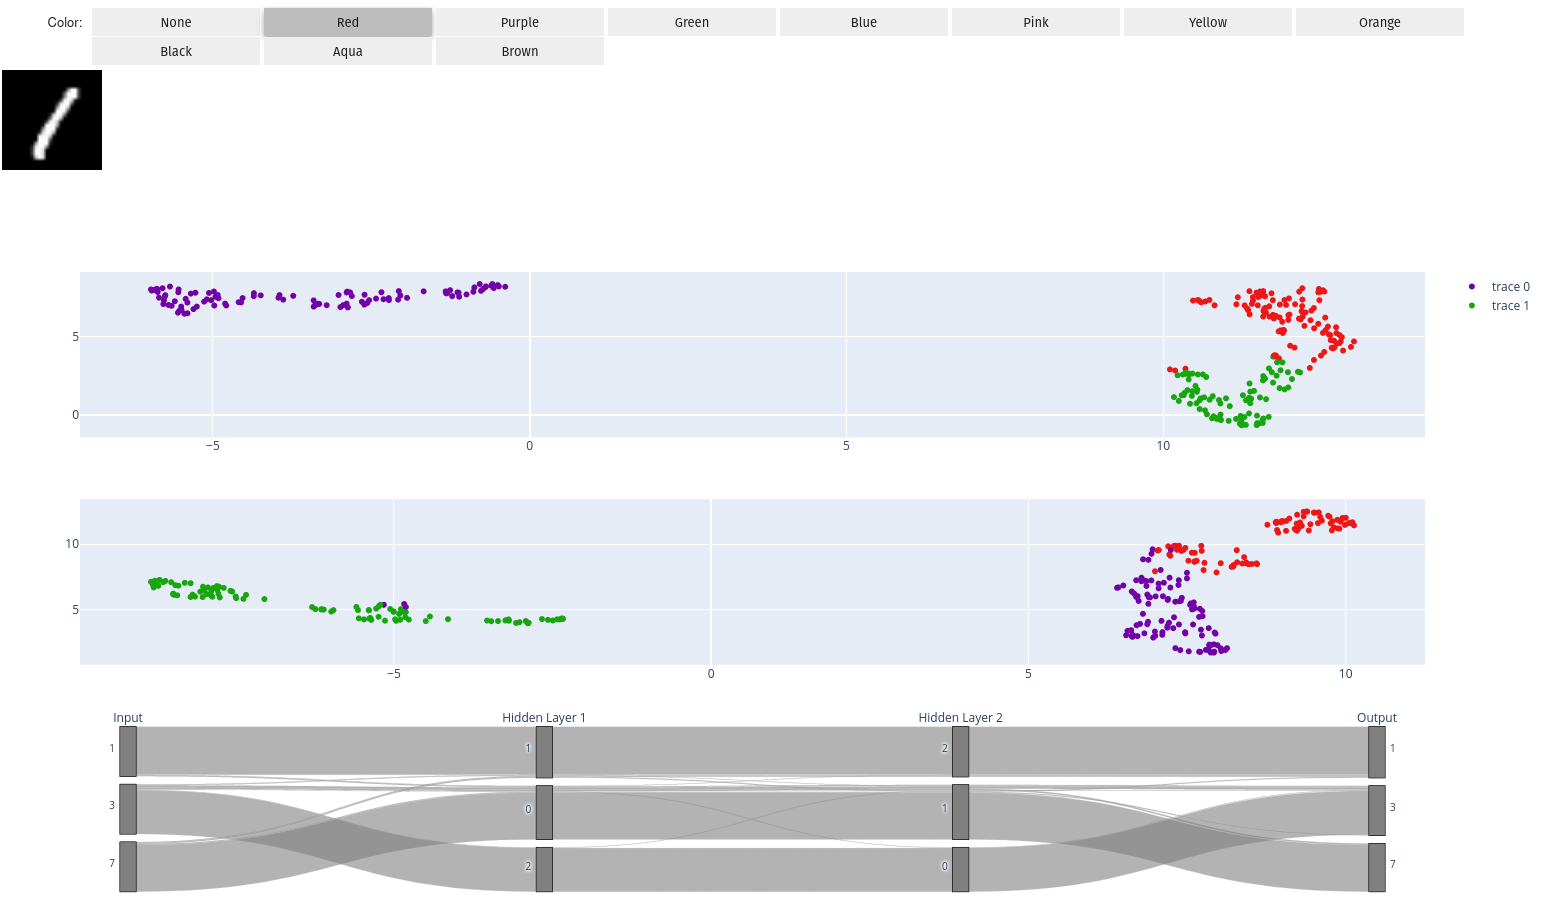
\includegraphics[width=0.8\textwidth]{img/umap-sankey2.png}}
\end{frame}

\begin{frame}{Application web}
    \begin{block}{Page d'accueil}
        Création d'une page d'accueil personnalisée présentant nos différentes expérimentations.
    \end{block}
    \makebox[\textwidth]{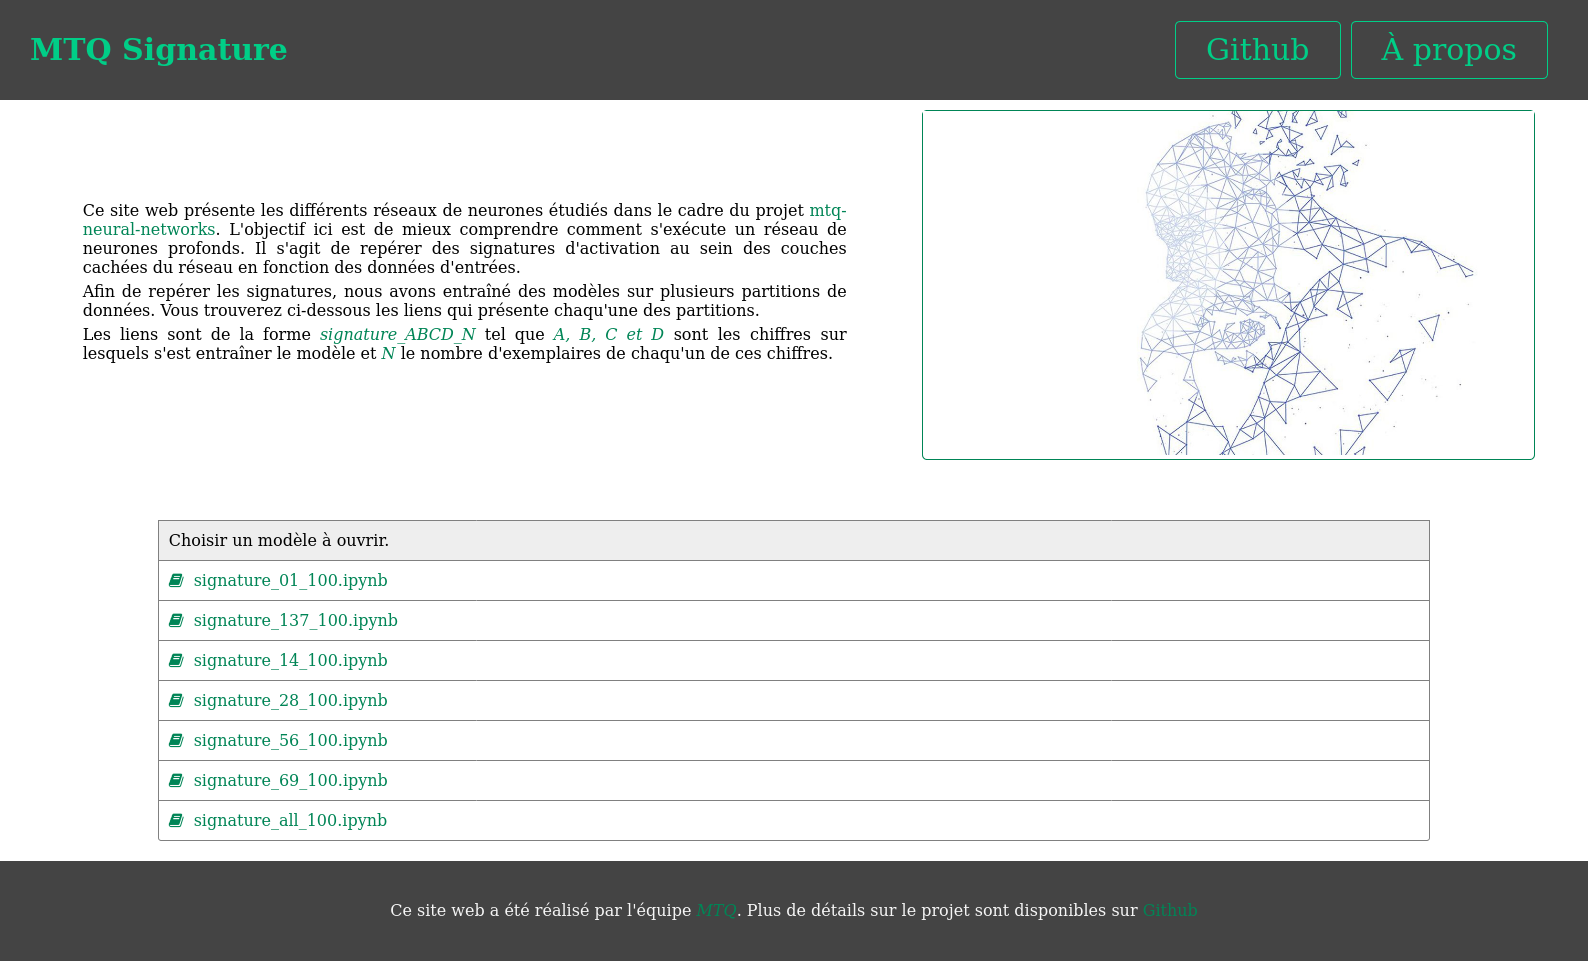
\includegraphics[width=0.8\textwidth]{img/accueil.png}}
\end{frame}
\placelogotrue

\section{Analyse des résultats}

\placelogofalse
\begin{frame}{Résultats}
    \makebox[\textwidth]{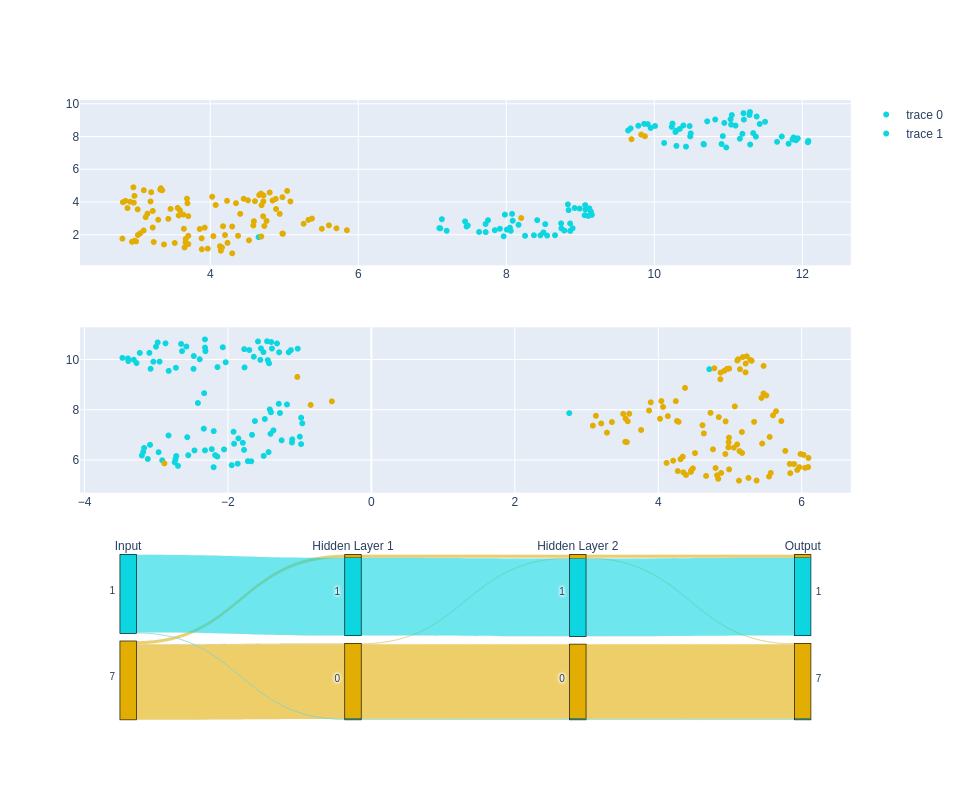
\includegraphics[width=0.8\textwidth]{img/visualisation17.png}}
\end{frame}
\placelogotrue

\subsection{Réponses aux questions}
\begin{frame}{Changement de comportement}
    %À partir de quelle couche le modèle change de comportement pour reconnaître une image ?
    \begin{block}{}
        Notre modèle arrive, dès la première couche cachée, à reconnaître une image.
    \end{block}
    
    \makebox[\textwidth]{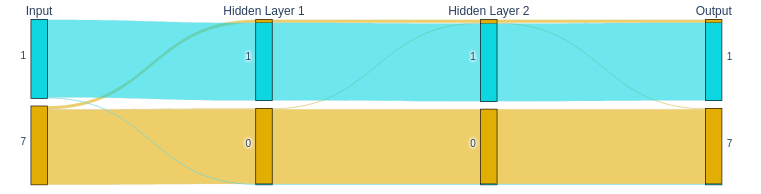
\includegraphics[width=0.8\textwidth]{img/sankey17.png}}
\end{frame}

\begin{frame}{Différence de signatures}
    %Les signatures des images de 7, sont-elles différentes de ceux des 1 ?
    \begin{block}{}
        On observe que les signatures des 1 sont majoritairement différentes de celles des 7. Sauf pour quelques rares exceptions.
    \end{block}

    \makebox[\textwidth]{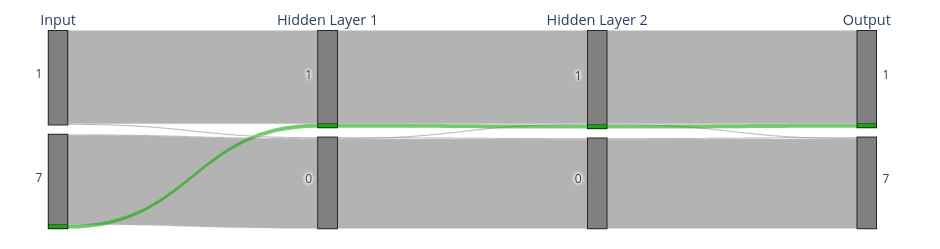
\includegraphics[width=0.8\textwidth]{img/sankey_7.png}}

\end{frame}

\begin{frame}
    \begin{figure}[h]
        \begin{minipage}[c]{.46\linewidth}
        \centering
        
\includegraphics[width=0.4\textwidth]{img/7_1.png}
        \end{minipage}
        \hfill%
        \begin{minipage}[c]{.46\linewidth}
        \centering
        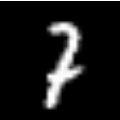
\includegraphics[width=0.4\textwidth]{img/7_2.png}
        \end{minipage}
        \end{figure}
        
        \begin{figure}[h]
        \begin{minipage}[c]{.46\linewidth}
        \centering
        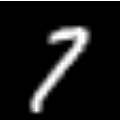
\includegraphics[width=0.4\textwidth]{img/7_3.png}
        \end{minipage}
        \hfill%
        \begin{minipage}[c]{.46\linewidth}
        \centering
        
\includegraphics[width=0.4\textwidth]{img/7_4.png}
        \end{minipage}
        \caption{Les images de 7 ressemblant à des 1}
        \label{71}
    \end{figure}
\end{frame}

\begin{frame}{Insertion d’anomalies}
    %Si on passe une image de 3 au modèle, à quoi va ressembler sa signature ?
    \begin{figure}[h]
        \centering
        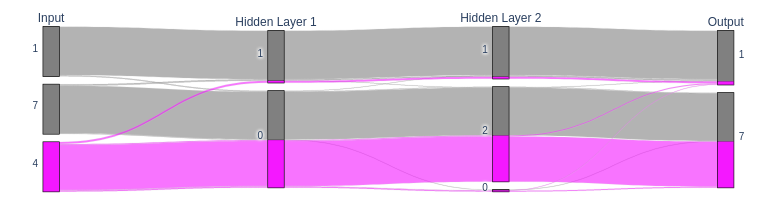
\includegraphics[width=0.9\textwidth]{img/anomalie4_sankey.png}
        \caption{Insertion d’images de 4}
    \end{figure}
\end{frame}

\begin{frame}{Insertion d’anomalies}
    %Si on passe une image de 3 au modèle, à quoi va ressembler sa signature ?
    \begin{figure}[h]
        \centering
        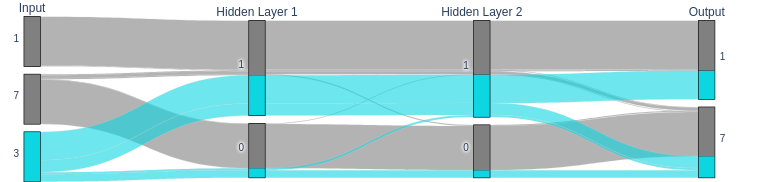
\includegraphics[width=0.9\textwidth]{img/anomalie3_sankey.png}
        \caption{Insertion d’images de 3}
    \end{figure}
\end{frame}

\section{Conclusion}
\begin{frame}{Conclusion}
    \begin{itemize}
        \item Un outil de visualisation ;
        \item Apports du projet ;
        \item Perspective.
    \end{itemize}
\end{frame}

\begin{frame}
    \begin{center}
      Merci pour votre attention.
    \end{center}
\end{frame}
  
\end{document}